



%----------------------------------------------------------------------------------------

\newpage

%%%%%%%%%%%%%%%%%%%%%%%
\section{Network growth heuristics}{Heuristiques de génération de réseau}

\label{app:sec:networkgrowth}




%%%%%%%%%%%%%%%%%
\begin{figure}
%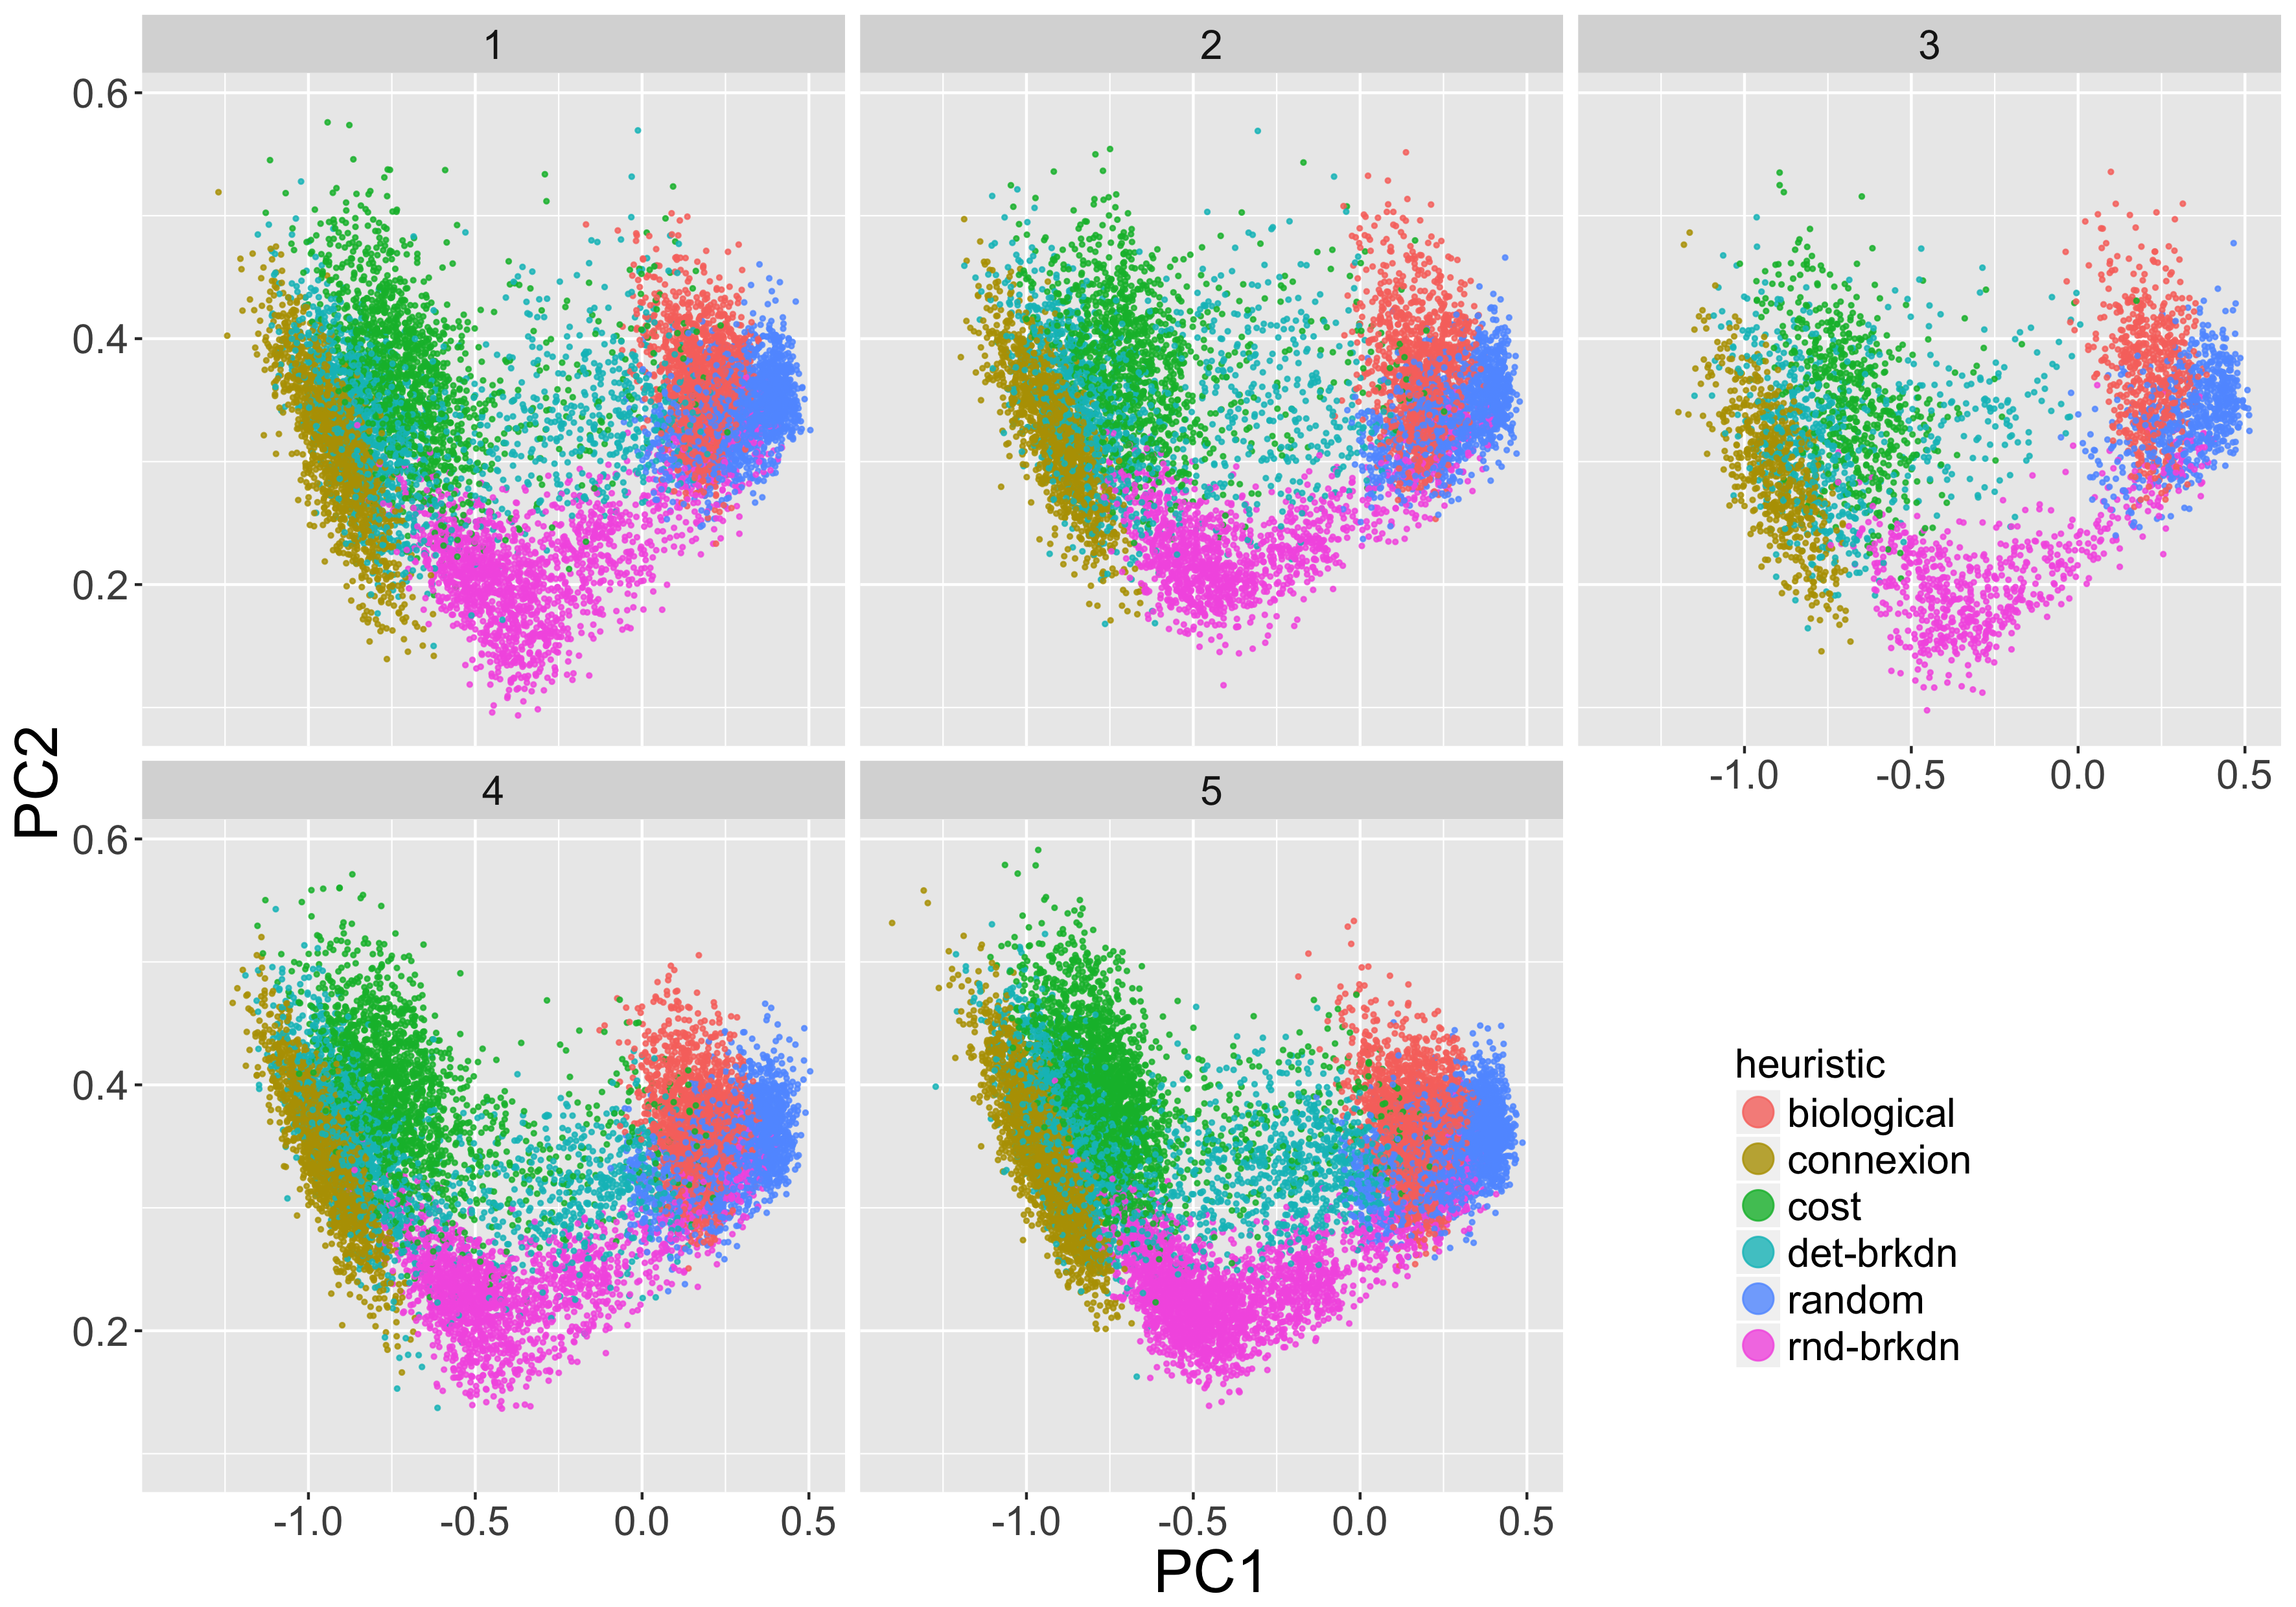
\includegraphics[width=\linewidth]{Figures/NetworkGrowth/feasible_space_pca_bymorph}
%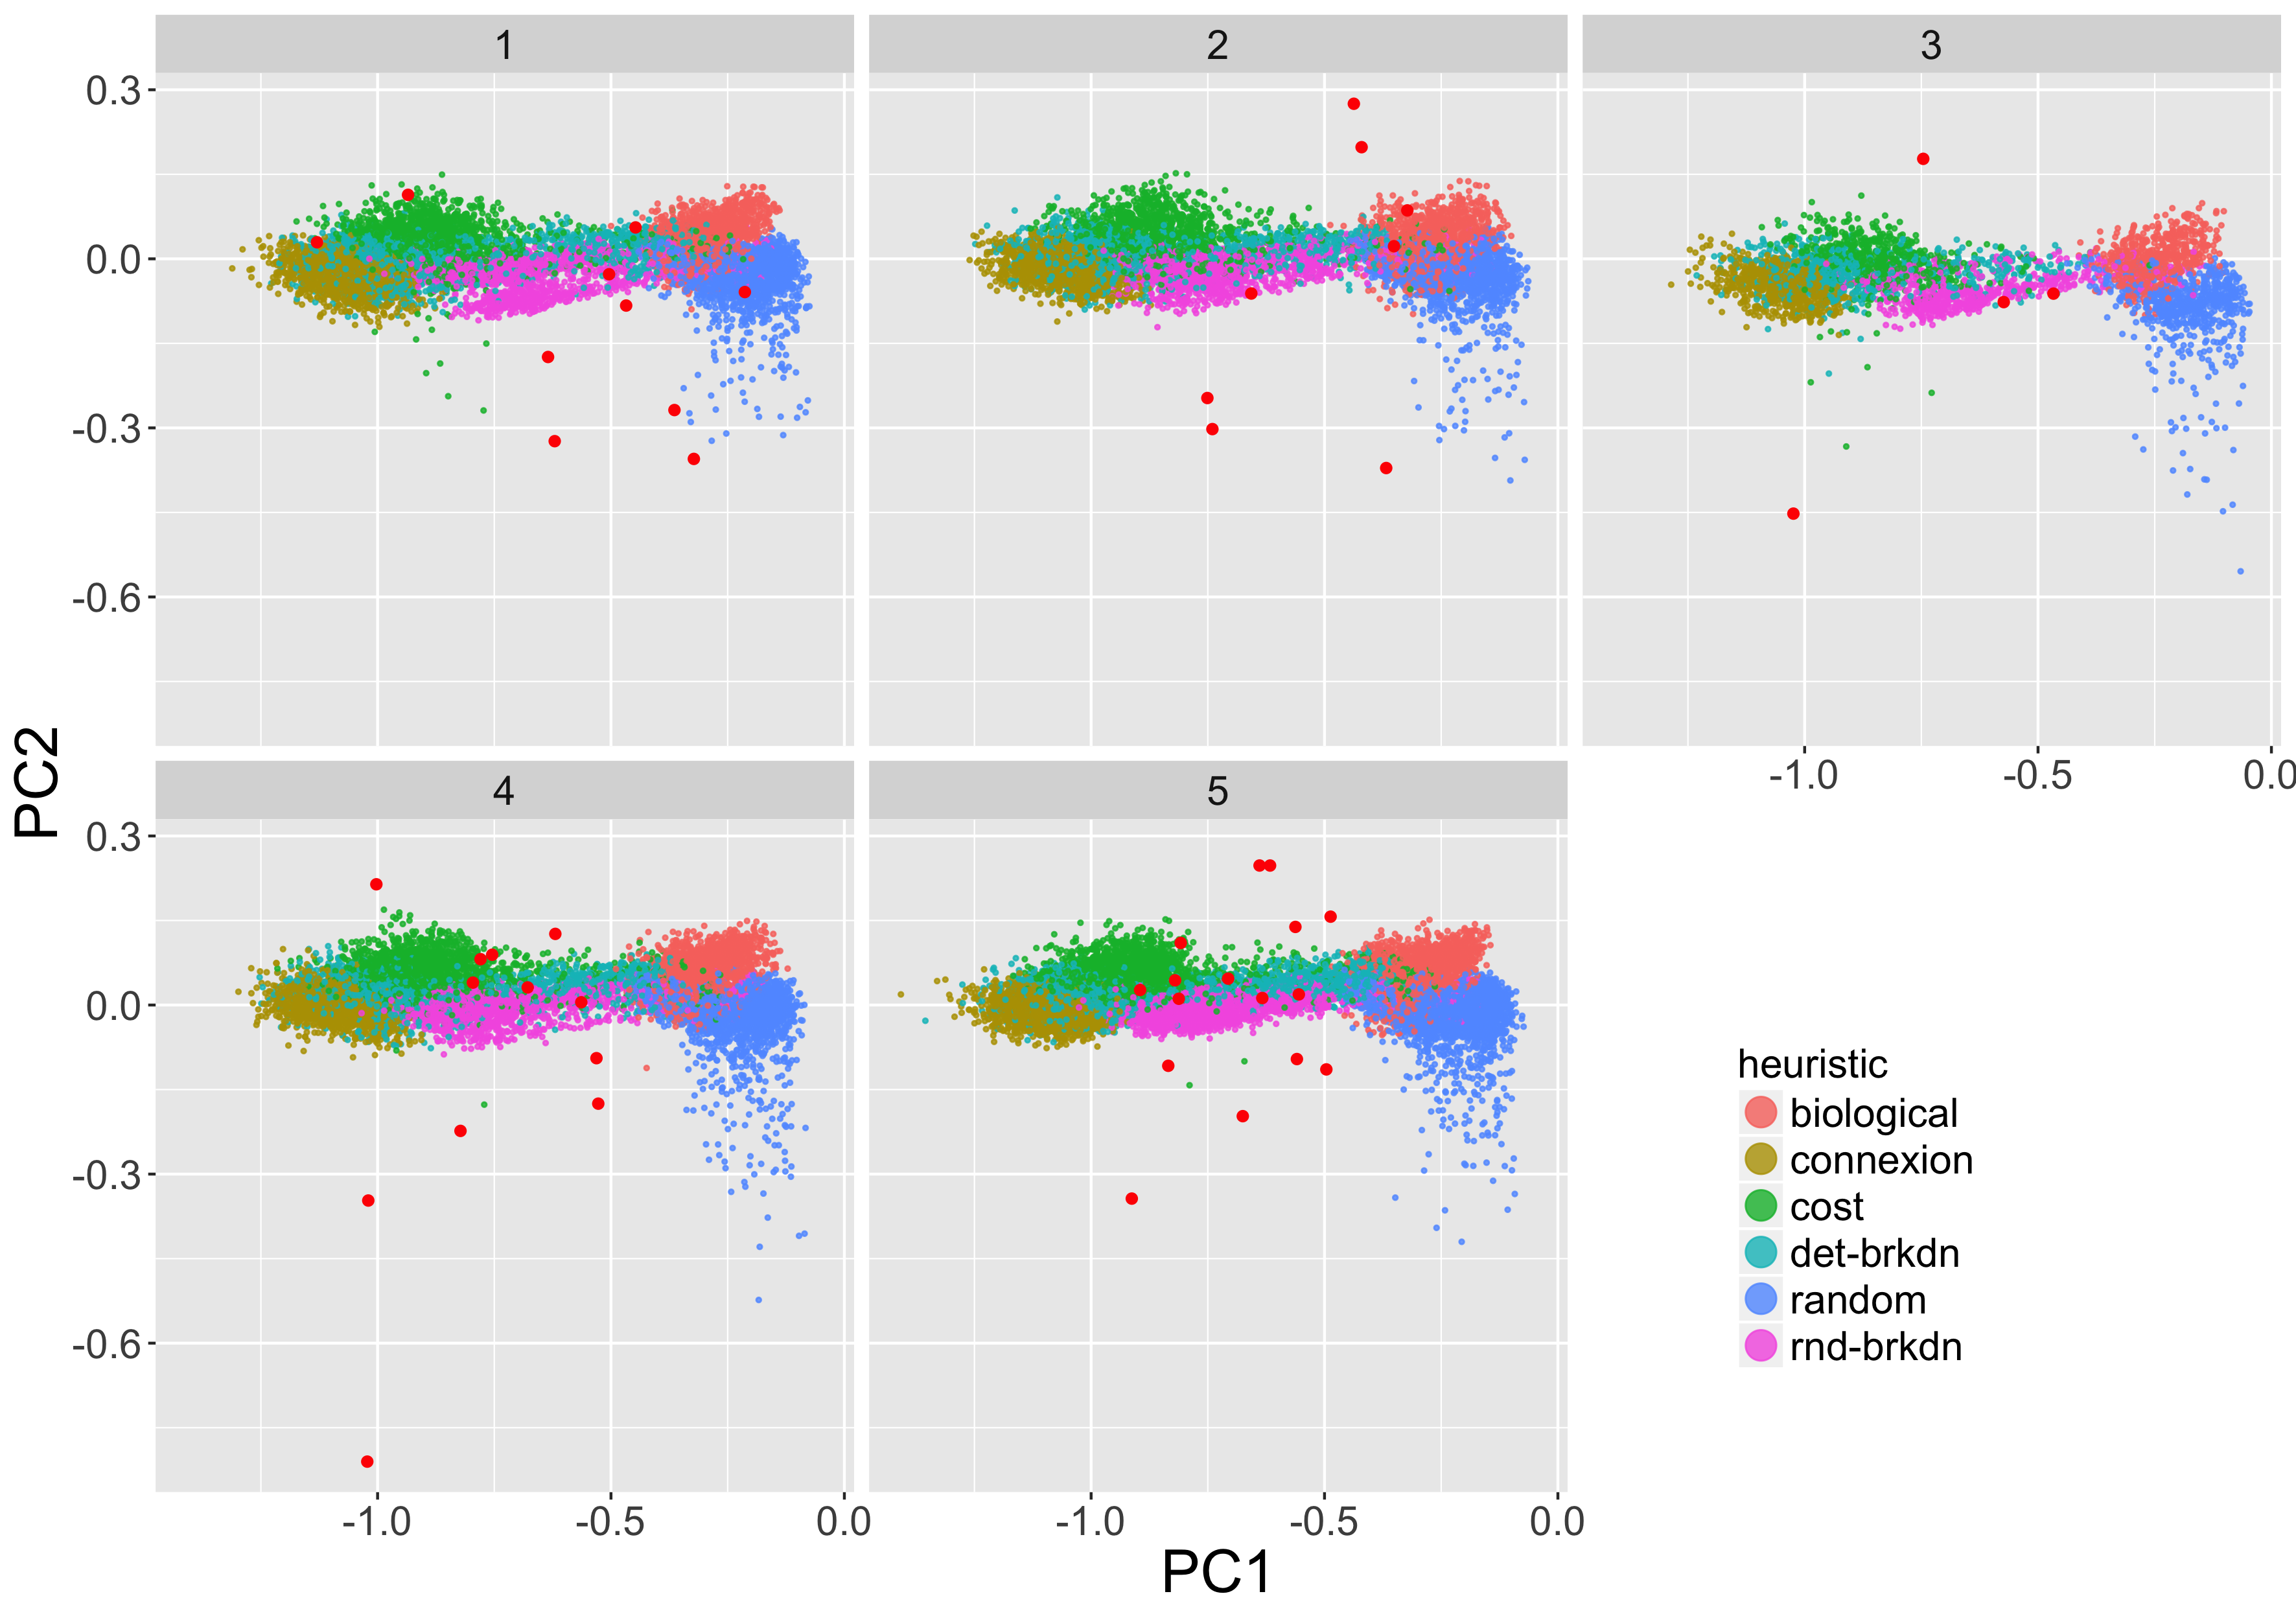
\includegraphics[width=\linewidth]{Figures/NetworkGrowth/feasible_space_withreal_pca_bymorph}
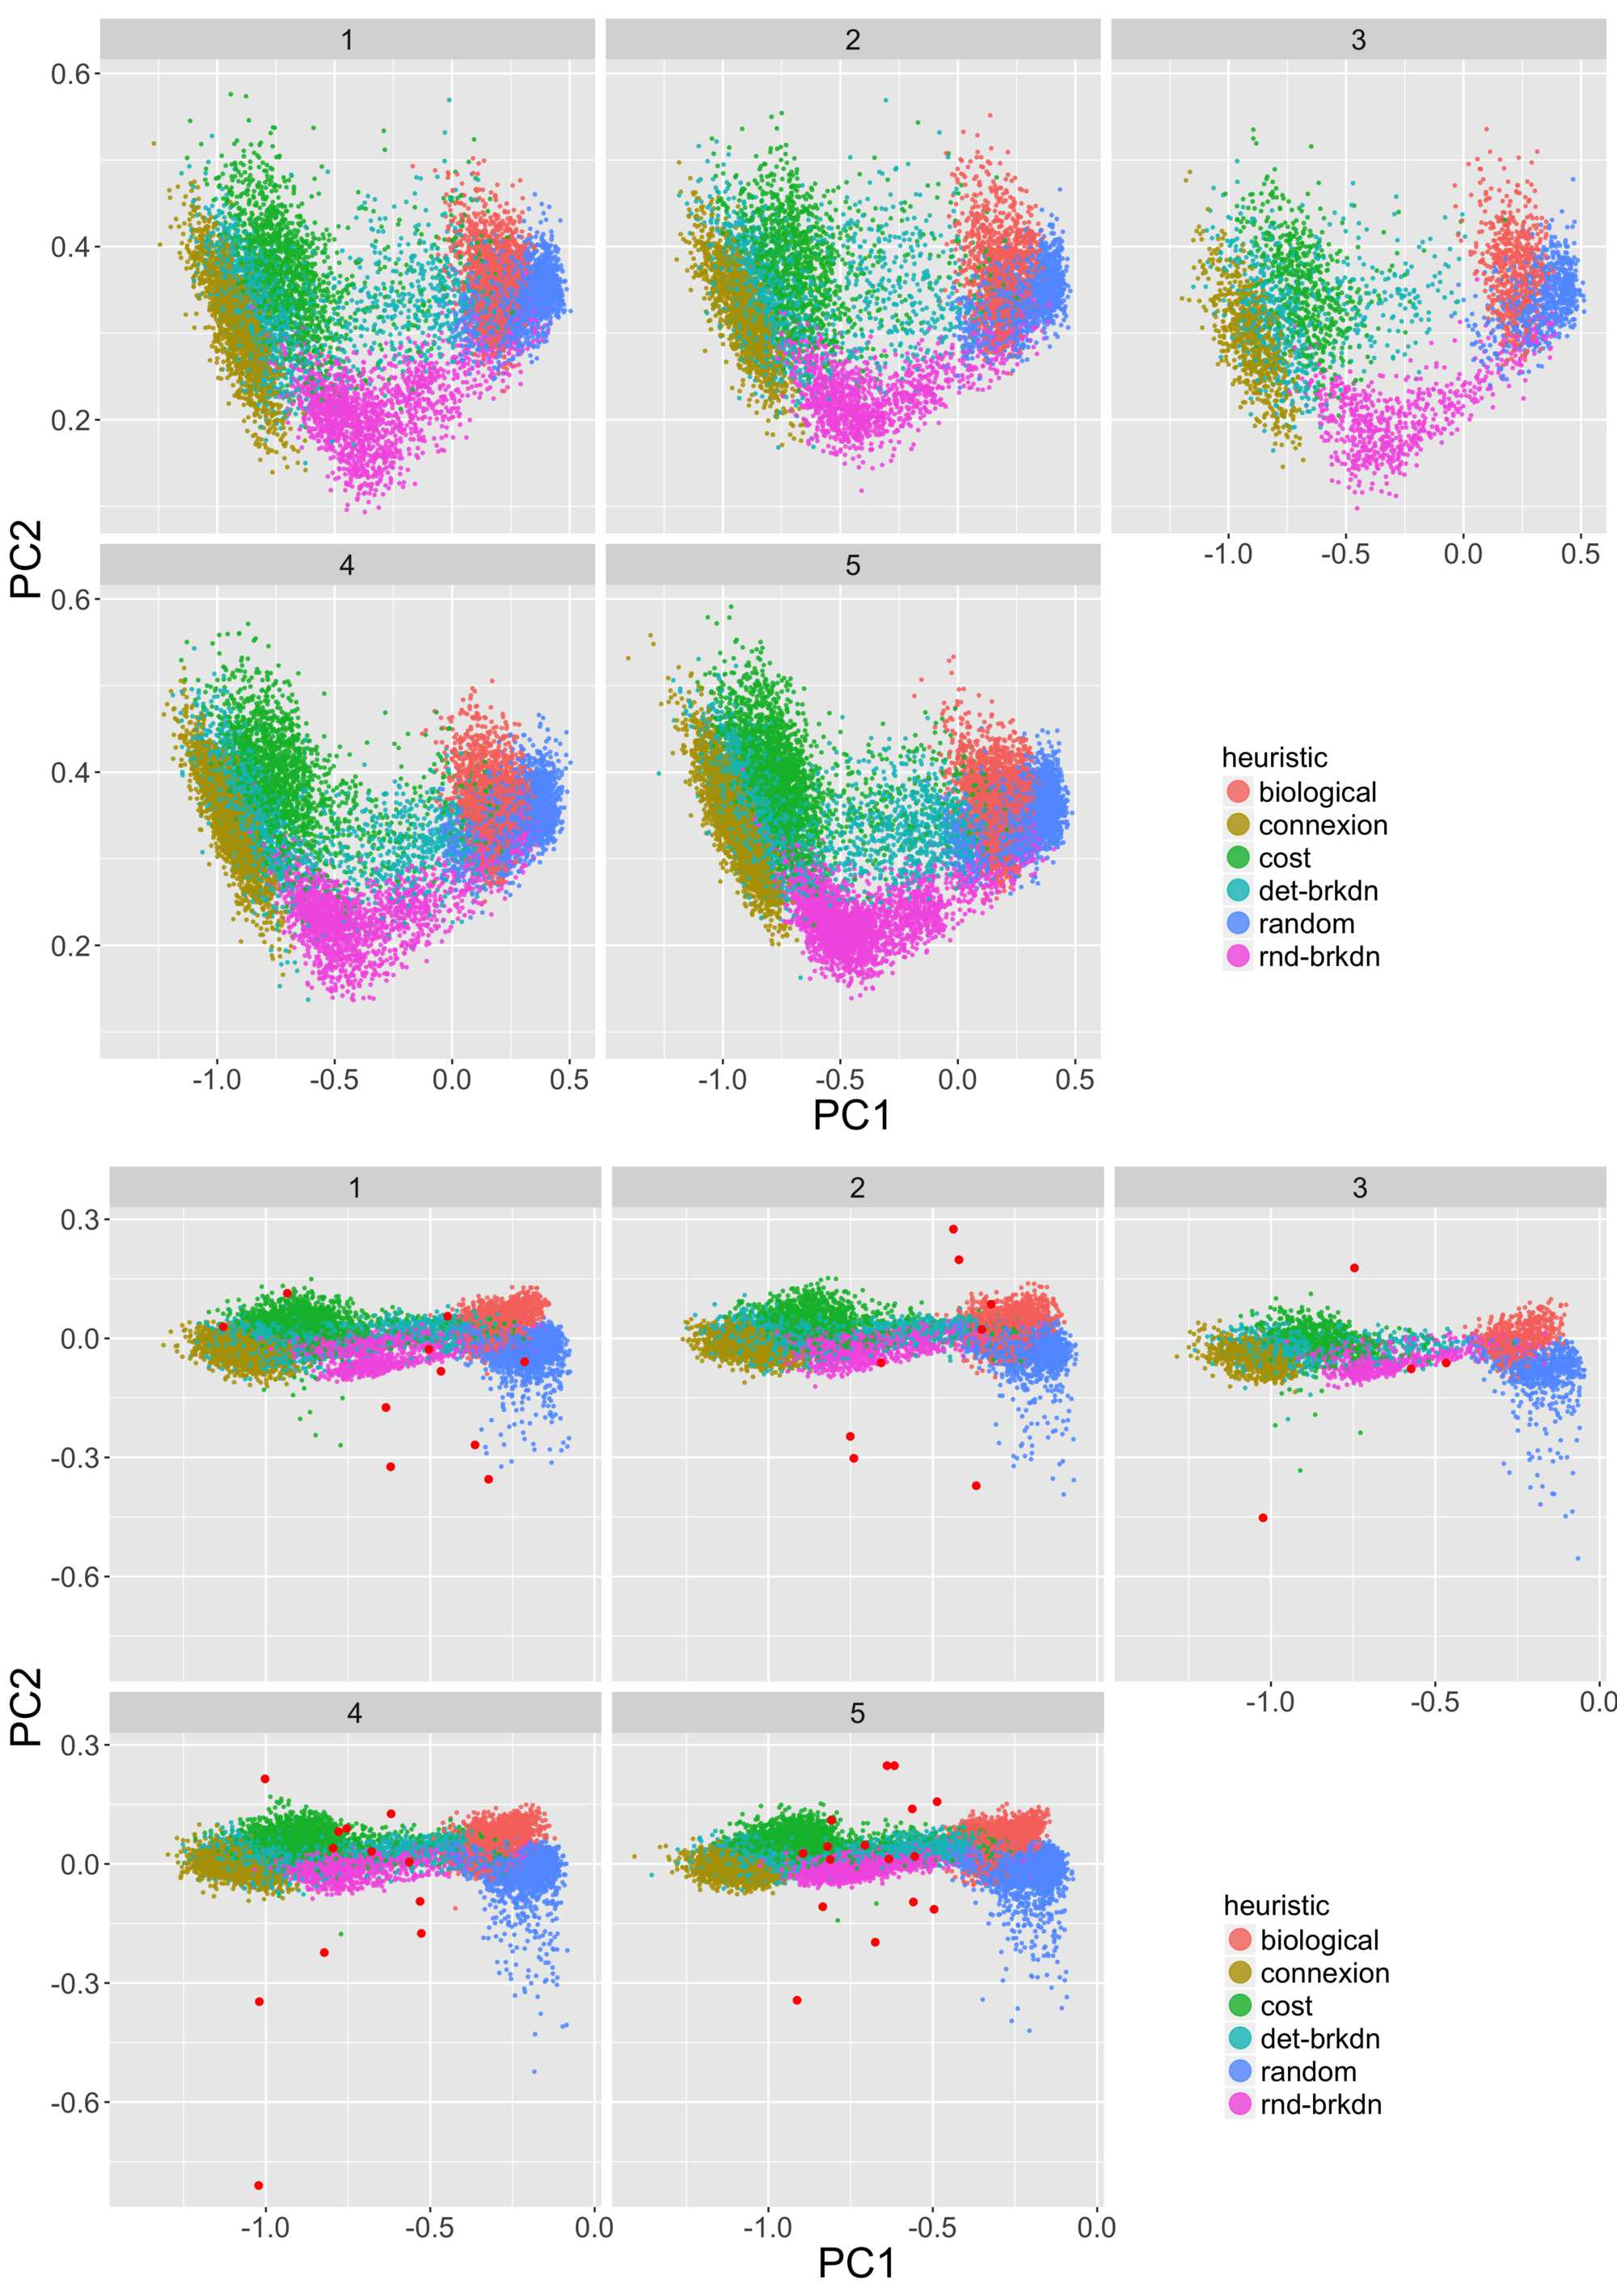
\includegraphics[width=0.9\linewidth]{Figures/Final/A-networkgrowth-feasiblespace_bymorph}
\appcaption{}{\textbf{Espace topologique faisable pour les différentes heuristiques de génération, conditionné à la classe morphologique de densité.}\label{fig:app:networkgrowth:feasiblespace_bymorph}}
\end{figure}
%%%%%%%%%%%%%%%%%














%----------------------------------------------------------------------------------------

\newpage

%%%%%%%%%%%%%%%%%%%%%%%
\section{Transportation Network Governance modeling}{Modélisation de la gouvernance du système de transport}



\subsection{Semi-analytical study of the land-use model}{Etude semi-analytique du modèle d'usage du sol}


Nous étudions ici la question de la convergence dans le temps de la distribution des activités.

Considérons un cas très simple : en prenant $\lambda = 0$ on déspatialise le problème et en prenant $\gamma_A = 1$ on finit de découpler population et emplois. En posant $\beta' = \sum_j E_j \cdot \beta$ et $P_0 = \frac{\sum_i P_i}{\sum_i \exp \beta' P_i}$, l'existence d'un point fixe pour les populations se ramène à la résolution de
\[
P_i = P_0 \cdot \exp\left(\beta' \cdot P_i\right)
\]


















